\documentclass[a4paper,12pt]{report}
\usepackage[a4paper, portrait, margin=0.5in]{geometry}
\usepackage[utf8]{inputenc}
\usepackage{graphicx}
\usepackage{dsfont}
\usepackage{amsmath}
\usepackage{esint}
\usepackage{mathtools}
\usepackage{cancel}
\usepackage{bbold}
\usepackage{wrapfig}
\usepackage{subcaption}
\usepackage{listings}
\usepackage{xcolor}		
\usepackage{systeme}
\usepackage{soul}
\usepackage{ amssymb }

\setcounter{secnumdepth}{3}
\setcounter{tocdepth}{3}

\newcommand{\limit}[2]{\underset{#1 \rightarrow #2}{\lim} \,}
\newcommand{\arrowlim}[2]{\overset{#1 \rightarrow #2}{\longrightarrow}}
\newcommand{\arrowlimtwo}[4]{\overset{\scriptsize{\begin{array}{cc}
				#1 {}&\rightarrow #2\\
				#3 &\rightarrow #4
		\end{array}}
	}{\longrightarrow}}

\newcommand{\Lagr}{\mathcal{L}}
\newcommand{\Four}{\mathcal{F}}
\newcommand{\TdZ}{\mathcal{Z}}
\newcommand{\R}{\mathbb{R}}
\newcommand{\C}{\mathbb{C}}
\newcommand{\N}{\mathbb{N}}
\newcommand{\Z}{\mathbb{Z}}
\newcommand{\nextpassage}{\nonumber \\ &\downarrow \nonumber \\}
\newcommand{\firstpassage}{ \\ &\downarrow \nonumber \\}
\newcommand{\spacer}{\quad ; \quad}
\newcommand{\except}[1]{\backslash \{ #1 \} }
\newcommand{\taleche}{\; : \;}
\newcommand{\bolditem}[1]{\item \textbf{#1}}
\newcommand{\separator}{\nonumber \\ 
	\nonumber \\}
\newcommand{\double}[2]{\left\{ \begin{array}{cc}
		#1\\
		#2
	\end{array}
	\right.
}
\newcommand{\triple}[3]{\left\{ \begin{array}{ccc}
		#1\\
		#2\\
		#3
	\end{array}
	\right.
}	
\newcommand{\quadruple}[4]{\left\{ \begin{array}{ccc}
		#1\\
		#2\\
		#3\\
		#4
	\end{array}
	\right.
}	

\newcommand{\nosgn}{\;\;\,}

\newcommand{\quadvec}[4]{\left( \begin{array}{ccc}
		#1\\
		#2\\
		#3\\
		#4
	\end{array}
	\right)
}

\newcommand{\circconv}{\underset{N}{\circledcirc}}
\newcommand{\dtftvar}{e^{j\omega t_s}}

% Title Page
\title{Realizzazione di un filtro Passa-Banda Chebyshev del 7° ordine}
\author{Alessandro Marcelli}


\begin{document}
\maketitle

\tableofcontents

\newpage

\section{Studio preliminare e descrizione della procedura}

La richiesta del progetto è di realizzare un filtro \textbf{Passa-Banda} Chebyshev di tipo 1 del 7° ordine  con le seguenti frequenze di taglio
\begin{align}
f_1 &= 26.5 \; MHz\\
f_2 &= 27.5  \; MHz
\end{align}

Dai valori assegnati ricaviamo le seguenti informazioni sul filtro
\begin{enumerate}
	\item Larghezza di banda passante
	\begin{align}
	\Delta f_{1,2} &= f_2 - f_1   =  1.00  \; MHz
	\end{align}
	
	\item Frequenza di media geometrica
	\begin{align}
	f_{mid} = \sqrt{f_1 \cdot f_2} \simeq 27.0 \; MHz
	\end{align}
	
	\item Larghezza di banda relativa
	\begin{align}
	\Delta f_{rel} =\frac{\Delta f_{1,2}}{f_{mid}} \simeq 0.04
	\end{align}
	
\end{enumerate}	

La progettazione e simulazione del filtro, fatta utilizzando SIMetrix, si snoda nei seguenti passaggi:
\begin{enumerate}
	\item Progettazione di un filtro \textbf{Passa-Basso} normalizzato del 7° ordine
	\item Denormalizzazione alla frequenza di taglio $f_c = 1.00 \; MHz$ e al carico di uscita di $50 \; \Omega$ (corrispondente all'ampiezza di banda del \textbf{Passa-Banda} desiderato), con simulazione per verificare il corretto funzionamento
	\item Trasformazione in \textbf{Passa-Banda} di quest'ultimo con opportuno cambio di variabile e conseguente simulazione
\end{enumerate}

\newpage

\section{Progettazione del Passa-Basso corrispondente}

Realizzare un filtro passivo di ordine $n$ \textbf{Passa-Basso} di Chebyshev significa volere una funzione di trasferimento normalizzata in frequenza tale che
\begin{align}
|H^{(n)}_{LP}(j\omega)|^2 = \frac{H_0^2}{1 + \epsilon^2 \cdot C_n^2(\omega)}
\end{align}

Dove
\begin{align}
\omega = 2\pi f
\end{align}

Le grandezze che caratterizzano il filtro sono dunque

\begin{enumerate}
	\item L'\textbf{amplificazione massima di banda passante} $H_0$, normalizzando rispetto alla quale si ottiene
	\begin{align}
	|N^{(n)}_{LP}(j\omega)|^2 = \frac{|H^{(n)}_{LP}(j\omega)|^2}{H_0^2} = \frac{1}{1 + \epsilon^2 \cdot C_n^2(\omega)}
	\end{align}
	
	Nel caso di filtri passivi questo valore non può superare 1, che corrisponde al caso ideale in assenza di perdite. 
	
	\item Il \textbf{fattore di ripple} $\epsilon$, il cui contributo all'\textbf{ampiezza massima in banda passante} $k_p$ viene descritto dalla seguente relazione
	\begin{align}
	k_p = 20 \cdot \log_{10} (\sqrt{1 + \epsilon^2}) \; [dB] 
	\end{align}
	
	Per questa esperienza si è scelto $\epsilon =1$, che restituisce
	\begin{align}
	k_p = 20 \cdot \log_{10} (\sqrt{2}) = 3 \; [dB] 
	\end{align}
	
	Questo valore si sposa bene con il valore della funzione di trasferimento tale in corrispondenza della pulsazione di taglio in $\omega_T=1$, dove
	\begin{align}
	|N^{(n)}_{LP}(j\omega_T)| = \frac{1}{\sqrt{2}}
	\end{align}
	
	Che corrisponde ad un'attenuazione di $3 \; [dB] $ rispetto all'ampiezza massima, permettendoci così di prendere la pulsazione di taglio come pulsazione di limite della banda passante.
	
	\item Il \textbf{polinomio di Chebyshev} $C_n(\omega)$, di ordine $n$ corrispondente a quello del filtro voluto. Tali polinomi sono definiti come
	\begin{align}
	C_n(\omega) = \double{\cos (n \cdot \arccos (\omega )) \quad &\omega \in [0,1]}{\cosh (n \cdot \text{arccosh} (\omega )) \quad &\omega \geq 1}
	\end{align}
	
	Nel nostro caso abbiamo bisogno di un polinomio del 6° ordine, che, consultando le tavole dei polinomi, risulta essere
	\begin{align}
	C_7(\omega) = 64\omega^7 - 112\omega^5 + 56\omega^3 -7\omega
	\end{align}
	
\end{enumerate}    

In base a quanto detto finora possiamo scrivere un primo abbozzo della funzione di trasferimento del filtro come
\begin{align}
|N^{(7)}_{LP}(j\omega)|^2 = \frac{1}{1 + (64\omega^7 - 112\omega^5 + 56\omega^3 -7\omega)^2}
\end{align}

Possiamo quindi procedere al calcolo dei poli.

Per i filtri Chebyshev si parte dalle seguenti espressioni
\begin{align}
&p_k = \sigma_k + j\omega_k \\
&\sigma_k = - \sin(u_k) \cdot \sinh (v)\\
&\omega_k = + \cos(u_k) \cdot \cosh (v)\\
&u_k = \frac{2k-1}{2n} \cdot \pi\\
&v = \frac{1}{n} \cdot \text{arcsinh} \left( \frac{1}{\epsilon} \right) \label{epsilon}
\end{align}

Nel nostro caso, dove abbiamo posto $n=7$ e $\epsilon =1$ avremo
\begin{align}
u_1 &= \frac{\pi}{14} \\
u_2 &= \frac{3}{14} \cdot \pi \\
u_3 &= \frac{5}{14} \cdot \pi\\
u_4 &= \frac{\pi}{2}\\
u_5 &= \frac{9}{14} \cdot \pi\\
u_6 &= \frac{11}{14} \cdot \pi\\
u_7 &= \frac{13}{14} \cdot \pi\\
v &= 0.1259
\end{align}

Da questi valori, tramite uno script in python creato ad hoc si è ottenuto
\begin{align}
&\double{\sigma_1 &= - \sin\left( \frac{\pi}{14} \right) \cdot \sinh \left( 0.1259 \right)}{\omega_1 &= + \cos\left( \frac{\pi}{14} \right) \cdot \cosh \left( 0.1259 \right)} \to &p_1 = -0.02809  +j \cdot  0.9827\\
\nonumber\\
&\double{\sigma_2 &= - \sin\left( \frac{3}{14} \cdot \pi \right) \cdot \sinh \left( 0.1259 \right)}{\omega_2 &= + \cos\left( \frac{3}{14} \cdot \pi \right) \cdot \cosh \left( 0.1259 \right)} \to &p_2 = -0.07871  +j \cdot 0.7880\\
\nonumber\\
&\double{\sigma_3 &= - \sin\left(\frac{\pi}{2} \right) \cdot \sinh \left( 0.1259 \right)}{\omega_3 &= + \cos\left( \frac{\pi}{2}\right) \cdot \cosh \left( 0.1259 \right)} \to &p_3 = -0.1137  +j \cdot 0.4373\\
\nonumber\\
&\double{\sigma_4 &= - \sin\left( \frac{9}{14} \cdot \pi \right) \cdot \sinh \left(  0.1259 \right)}{\omega_4 &= + \cos\left( \frac{9}{14} \cdot \pi \right) \cdot \cosh \left(  0.1259 \right)} \to
&p_4 = -0.1262\\
\nonumber\\
&\double{\sigma_5 &= - \sin\left( \frac{9}{14} \cdot \pi \right) \cdot \sinh \left( 0.1259 \right)}{\omega_5 &= + \cos\left( \frac{9}{14} \cdot \pi \right) \cdot \cosh \left( 0.1259 \right)} \to
&p_5 = -0.11374  -j \cdot 0.4373\\
\nonumber\\
&\double{\sigma_6 &= - \sin\left( \frac{11}{14} \cdot \pi \right) \cdot \sinh \left(0.1259 \right)}{\omega_6 &= + \cos\left( \frac{11}{14} \cdot \pi \right) \cdot \cosh \left( 0.1259 \right)} \to
&p_6 = -0.078711  -j \cdot 0.7880\\
\nonumber\\
&\double{\sigma_7 &= - \sin\left( \frac{13}{14} \cdot \pi \right) \cdot \sinh \left(0.1259 \right)}{\omega_7 &= + \cos\left( \frac{13}{14} \cdot \pi \right) \cdot \cosh \left( 0.1259 \right)} \to
&p_7 = -0.02809  -j \cdot 0.9827
\end{align}

\newpage
Abbiamo quindi 7 poli disposti lungo un ellisse, di cui 6 simmetrici rispetto all'asse reale, come ci si aspetta dai filtri Chebyshev
\begin{figure}[!htb]
	\centering
	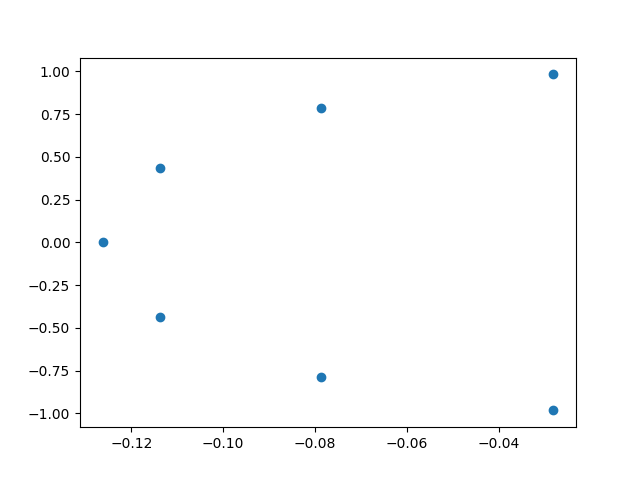
\includegraphics[width=.4\textwidth]{n=7_epsilon=1.0.png}
	\label{lol}
	\caption{\label{kekw} \small Poli del filtro}
\end{figure}

La presenza di sette poli si traduce nella progettazione circuitale in sette componenti passive reattive. In questo caso si è optato per una configurazione a scala con quattro condensatori e tre induttori.

Il calcolo dei valori per le componenti è passato per la consultazione della tavola di Chebyshev per ripple a $3 \; dB$. 
\begin{figure}[!htb]
	\centering
	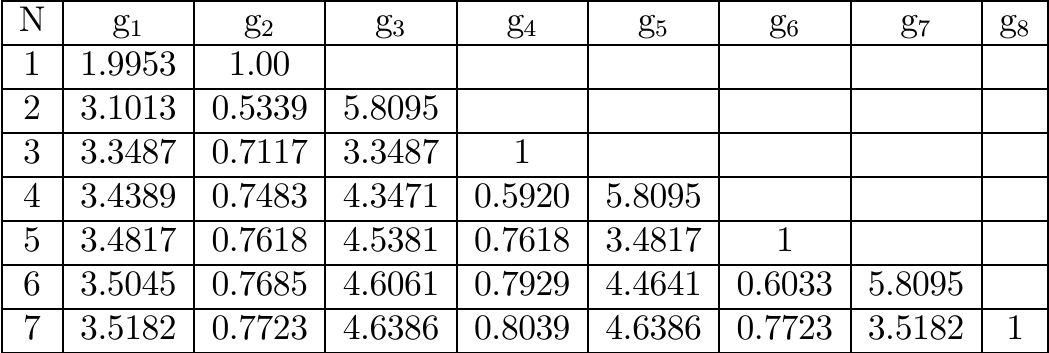
\includegraphics[width=.6\textwidth]{table.png}
	\label{loll}
	\caption{\label{kikw} \small Tabella delle impedenze normalizzate per filtri Chebyshev con ripple da $3 \; dB$}
\end{figure}

Dalla tabella, facendo corrispondere i valori per le capacità ai termini dispari e quelli per le induttanze a quelli pari, e sapendo che l'ultimo termine riguarda il carico si sono ottenuti i seguenti valori per il filtro normalizzato
\begin{center}
	\begin{tabular}{||c c c c c c c c ||} 
		\hline
		$C_2$  & $L_2$  & $C_3$  & $L_3$  & $C_4$  & $L_4$  & $C_1$  & $Z_{out}$\\ [0.5ex] 
		\hline\hline
		3.5182 & 0.7723 & 4.6386 & 0.8039 & 4.6386 & 0.7723 & 3.5182 & 1.0000\\ 
		\hline
	\end{tabular}
\end{center}


Questi valori sono stati poi denormalizzati per adeguarsi alla nostra frequenza taglio $f_c = 1 \; MHz$ e al carico di nostro interesse di $Z_0 = 50 \; \Omega$ tramite le seguenti relazioni
\begin{align}
C_i &= \frac{C_{i_{norm}}}{Z_0 \cdot 2\pi \cdot f_c}\\
L_i &= \frac{L_{i_{norm}}\cdot Z_0}{2\pi \cdot f_c}\\
R_o &= g_8 \cdot Z_0
\end{align}

Facendo uso di un altro script in python anch'esso scritto per l'evenienza si sono così ottenuti i seguenti valori
\begin{center}
		\begin{tabular}{||c c c c c c c c||} 
		\hline
		$C_2 \;[nF]$  & $L_2 \;[\mu H]$  & $C_3 \;[nF]$  & $L_3 \;[\mu H]$  &$C_4 \;[nF]$  & $L_4 \;[\mu H]$  & $C_1 \;[nF]$  & $Z_{out} 	\;[\Omega]$\\ [0.5ex] 
		\hline\hline
		11.199 & 6.1458 & 14.765 & 6.3972 & 14.765 & 6.1458 & 11.199 & 50.000\\ 
		\hline
	\end{tabular}
\end{center}
\newpage

Abbiamo quindi costruito il seguente filtro \textbf{Passa-Basso}

\begin{figure}[!htb]
	\centering
	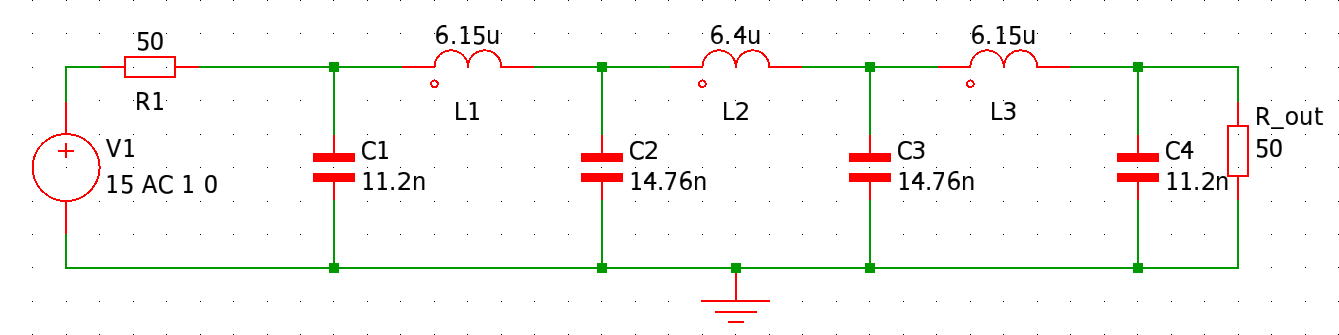
\includegraphics[width=\textwidth]{passa_basso.png}
	\label{lel}
	\caption{\label{kokw} \small Passa-Basso risultante}
\end{figure}

Il filtro così progettato risponde alle aspettative, infatti come vediamo dai diagrammi di Bode, alla frequenza $1 \; MHz$ si ha un valore del rapporto ingresso-uscita di circa $0.7$, che corrisponde ad un'attenuazione di circa $3 \; dB$, ovvero l'attenuazione che ci si aspetta alla frequenza di taglio, e la massima ampiezza picco-picco è di circa $1.5$, o, convertendo in Decibel, $3.5 \; dB$, abbastanza vicino al valore ideale.

Sono anche evidenti i 5 picchi previsti da un filtro del settimo ordine.

\begin{figure}[!htb]
	\centering
	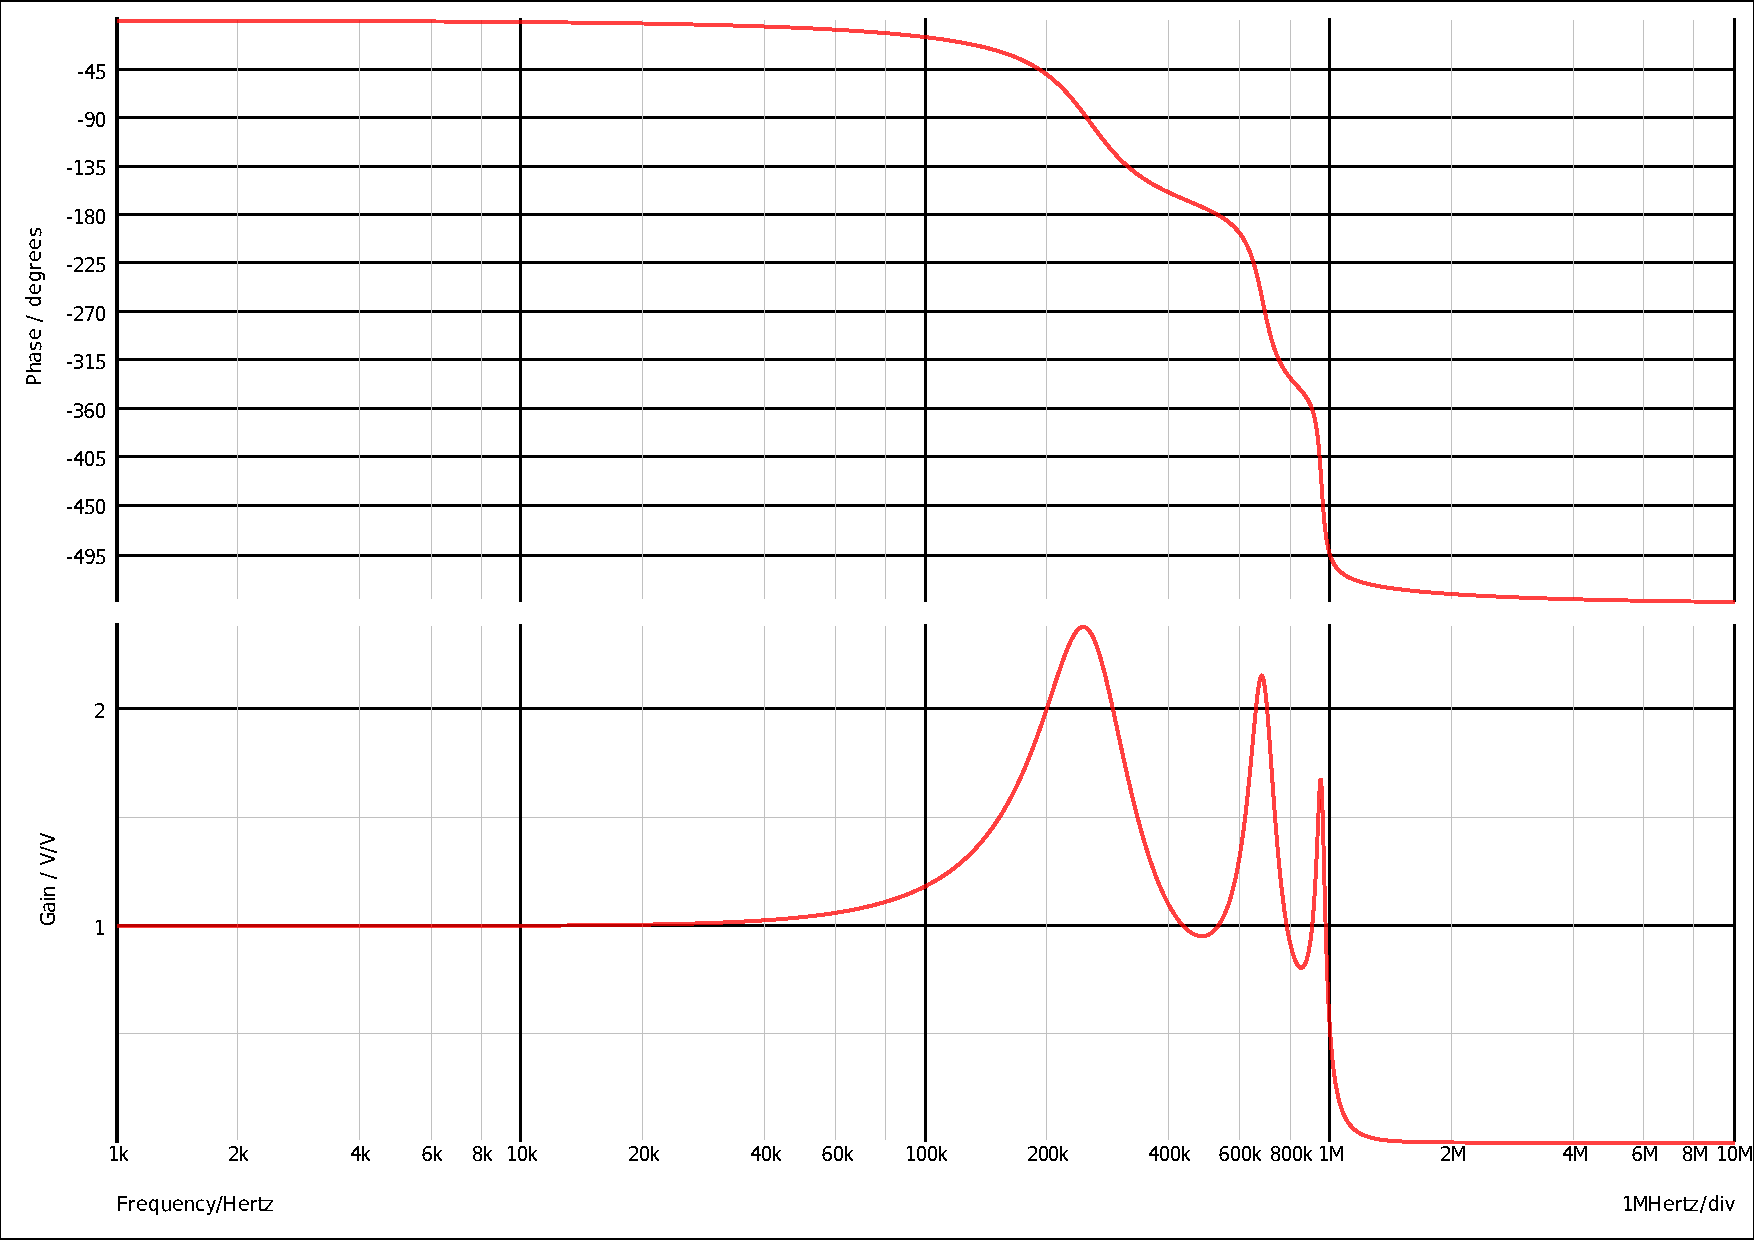
\includegraphics[width=.7\textwidth]{bodeesame1.pdf}
	\label{lel}
	\caption{\label{kokw} \small Diagrammi di Bode del filtro Passa-Basso}
\end{figure}

\newpage

\section{Realizzazione del Passa-Banda}

Matematicamente, la trasformazione da \textbf{Passa-Basso} a \textbf{Passa-Banda} prevede il seguente cambio di variabili
\begin{align}
&s = p + \frac{1}{p} = \frac{p^2 + 1}{p} \spacer p\in \C \firstpassage
&p = \frac{s}{2} \pm \sqrt{\left(\frac{s}{2}\right)^2 - 1}\\
\nonumber\\
&s = \sigma \pm j \omega\\
&p = u + jv
\end{align}

Essendo noi interessati all'analisi in frequenza possiamo restringere le variabili al caso puramente immaginario
\begin{align}
&s = \pm j\omega\\
&p = +jv
\end{align}

Ottenendo così
\begin{align}
&v_{1,2} = \frac{\omega}{2} \pm \sqrt{\left(\frac{\omega}{2}\right)^2 + 1}
\end{align}

Dove $v_1$ e $v_2$ sono le \textbf{frequenze di taglio} del nuovo filtro \textbf{Passa-Banda}.

Questo cambio di variabile nella progettazione del filtro si traduce in
\begin{enumerate}
	\item mettere in serie agli induttori del \textbf{Passa-Basso} dei condensatori
	\item mettere in parallelo ai condensatori del \textbf{Passa-Basso} degli induttori
\end{enumerate}

I valori di queste nuove componenti si calcolano tramite le seguenti relazioni:
\begin{align}
&L_{k_{//}} = \frac{\Delta f_{rel} \cdot Z_0}{2\pi\cdot f_{mid} \cdot C_{k_{norm}}}\\
&C_{k_{serie}} = \frac{\Delta f_{rel}}{2\pi\cdot f_{mid} \cdot L_{k_{norm}} \cdot Z_0}
\end{align}

Abbiamo definito $\Delta f_{rel}$ e $f_{mid}$ nel primo paragrafo di questo testo, e i valori normalizzati sono gli stessi delle equazioni (35)-(42) di pag. 6.

Sempre tramite custom script in python si sono ottenuti i seguenti valori:
\begin{align}
L_{1_{//}} &= 3.10 \; nH\\
L_{2_{//}} &= 2.35 \; nH\\
L_{3_{//}} &= 2.35 \; nH\\
L_{4_{//}} &= 3.10 \; nH\\
C_{1_{serie}} &= 5.65 \; pF\\
C_{2_{serie}} &= 5.43 \; pF\\
C_{3_{serie}} &= 5.65 \; pF
\end{align}

\newpage

Si è quindi raddoppiato il numero di componenti, con quattro nuovi induttori e tre nuovi condensatori, portandoci ad avere la seguente configurazione:
\begin{figure}[!htb]
	\centering
	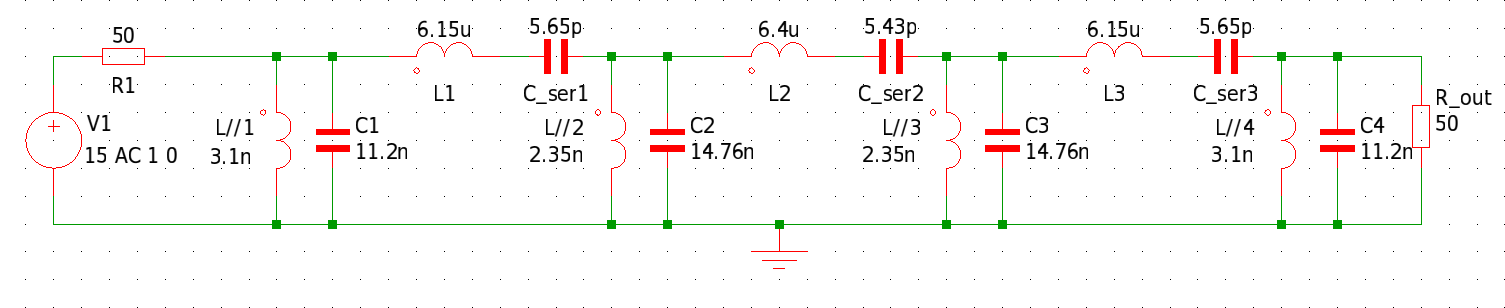
\includegraphics[width=\textwidth]{passa_banda.png}
	\label{lelz}
	\caption{\label{kokwz} \small Passa-Banda}
\end{figure}


Di seguito sono riportati i diagrammi di Bode del filtro, la cui risposta soddisfa i parametri di progettazione.

\begin{figure}[!htb]
	\centering
	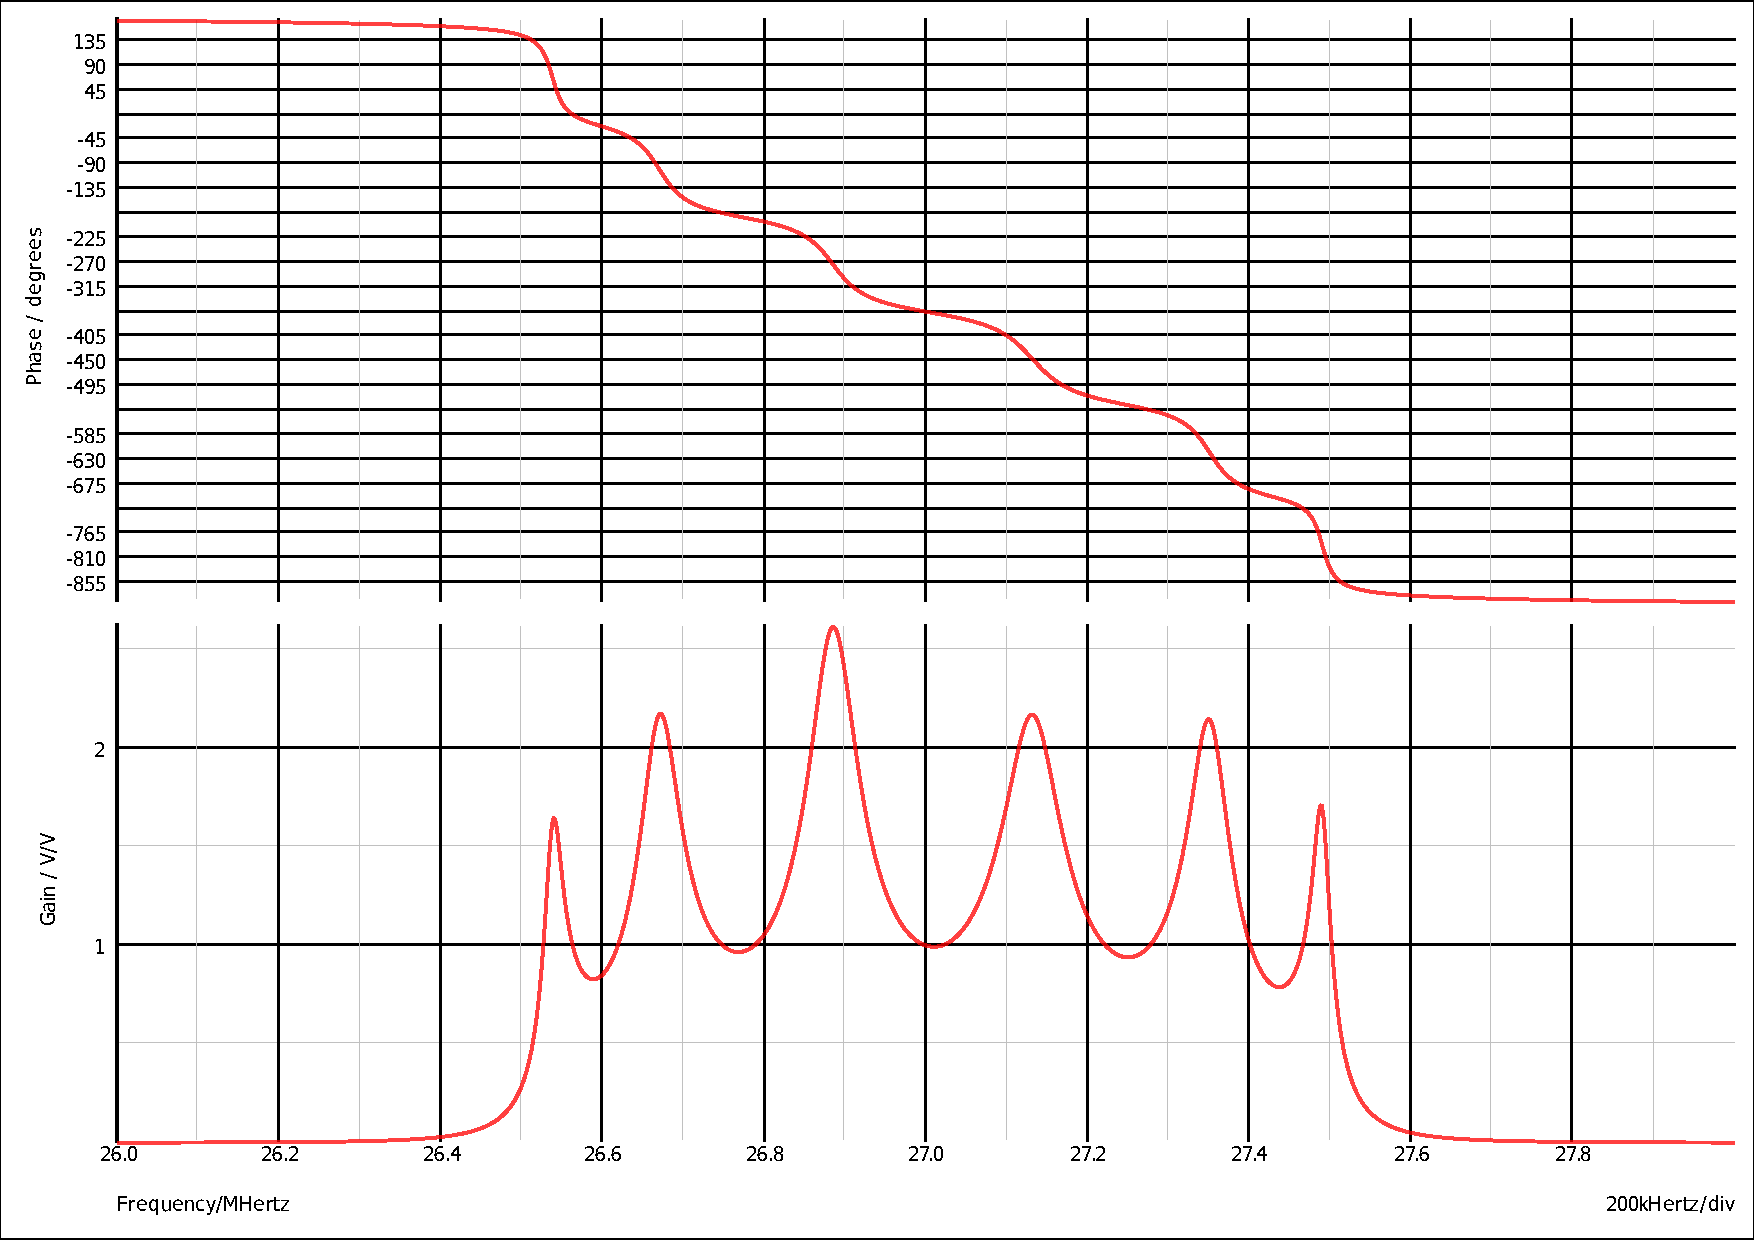
\includegraphics[width=.7\textwidth]{bodeesame21.pdf}
	\label{lell}
	\caption{\label{koklw} \small Diagrammi di Bode del Passa-Banda}
\end{figure}

Abbiamo infatti alle frequenze di taglio usate per la progettazione un valore del rapporto ingresso-uscita di circa $0.7$, ovvero circa $\frac{1}{\sqrt{2}}$, mentre l'ampiezza di ripple è analoga al Passa-Basso progettato in precedenza, intorno ai $3.5 \; dB$.

\section{Conclusioni}

In questo breve lavoro è stata presentata la progettazione di un filtro \textbf{Passa-Banda} del 7° ordine di Chebyshev tipo 1, con frequenze di taglio $26.5 \; MHz$ e $27.5 \; MHz$. 
Salvo inevitabili approssimazioni numeriche del software di simulazione il risultato è sostanzialmente in accordo con le previsioni teoriche.

\end{document}